\documentclass[journal]{IEEEtran}
\usepackage[a5paper, margin=10mm, onecolumn]{geometry}
\usepackage{tfrupee} 

\setlength{\headheight}{1cm}
\setlength{\headsep}{0mm} 

\usepackage{gvv-book}
\usepackage{gvv}
\usepackage{amsmath,amssymb,amsfonts,amsthm}
\usepackage{algorithmic}
\usepackage{graphicx}
\usepackage{textcomp}
\usepackage{xcolor}
\usepackage{txfonts}
\usepackage{listings}
\usepackage{enumitem}
\usepackage{mathtools}
\usepackage{gensymb}
\usepackage{comment}
\usepackage[breaklinks=true]{hyperref}
\usepackage{tkz-euclide} 
\usepackage{listings}
\def\inputGnumericTable{}                      
\usepackage[latin1]{inputenc}                                
\usepackage{color}                                         

\usepackage{array}                                            
\usepackage{longtable}                                       
\usepackage{calc}                 

\usepackage{multirow}                                         
\usepackage{hhline}                               
\usepackage{ifthen}                            
               
\usepackage{lscape}
\usepackage{tikz}
\usepackage[compatibility=false]{caption}

\usetikzlibrary{patterns}
\begin{document}


\vspace{3cm}


\title{GATE 2025 - General Aptitude \& Ecology and Evolution (EY)}
\author{ee25btech11034-Kishora Karthik}
\maketitle

{\let\newpage\relax\maketitle}

\renewcommand{\thefigure}{\theenumi}
\renewcommand{\thetable}{\theenumi}
\setlength{\intextsep}{10pt} 

\section*{\textbf{General Aptitude}}
\textbf{Q.1 - Q.5 Multiple Choice Question (MCQ), carry ONE mark each (for each wrong answer: $-1/3$).}
 
\begin{enumerate}
    \item Here are two analogous groups, Group-I and Group-II, that list words in their decreasing order of intensity.
Identify the missing word in Group-II.
    \\
    Group-I: $Abuse \rightarrow Insult \rightarrow Ridicule$
    \\
    Group-II: $\underline{\hspace{2cm}} \rightarrow Praise \rightarrow Appreciate$
    \begin{multicols}{2}       
    \begin{enumerate}
        \item Extol
        \item Prize
        \item Appropriate
        \item Espouse
    \end{enumerate}
    \end{multicols}

    \item Had I learnt acting as a child, I 
\underline{\hspace{3cm}} a famous film star.
    \\
    Select the most appropriate option to complete the above sentence.
\begin{multicols}{2}
    \begin{enumerate}
        \item will be
        \item can be
        \item am going to be
        \item could have been
    \end{enumerate}
    \end{multicols}
    
    \item The $12$ musical notes are given as $C$, $C^{\#}$, $D$, $D^{\#}$, $E$, $F$, $F^{\#}$, $G$, $G^{\#}$, $A$, $A^{\#}$, and $B$.
Frequency of each note is $\sqrt[12]{2}$ times the frequency of the previous note.
If the frequency of the note $C$ is $130.8$ Hz, then the ratio of frequencies of notes $F^{\#}$ and $C$ is:
    \begin{multicols}{2}
    \begin{enumerate}
        \item $\sqrt[6]{2}$
        \item $\sqrt{2}$
        \item $\sqrt[4]{2}$
        \item $2$
    \end{enumerate}
    \end{multicols}

    \item The following figures show three curves generated using an iterative algorithm.
The total length of the curve generated after 'Iteration $n$' is:
    \\
    Note: The figures shown are representative.
    \clearpage
\begin{figure}[!h]
        \centering
        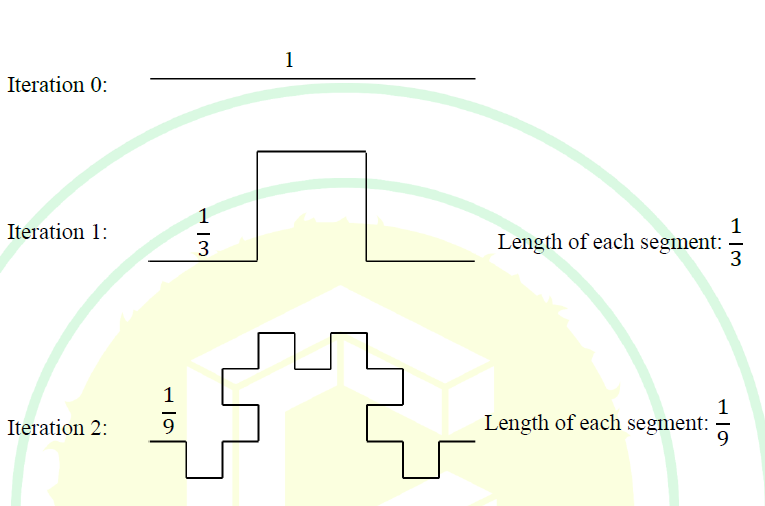
\includegraphics[width=0.4\columnwidth]{figs/Q.4.png}
        \caption{Curves generated by an iterative algorithm at Iteration 0, Iteration 1, and Iteration 2.}
        \label{fig:Q.4}
    \end{figure}
    \begin{multicols}{2}
    \begin{enumerate}
        \item $(\frac{5}{3})^{\frac{n}{2}}$
        \item $(\frac{5}{3})^{n}$
        \item $(\frac{5}{3})$
        \item $(\frac{5}{3})^{n(2n-1)}$
    \end{enumerate}
    \end{multicols}
    
    \item Which one of the following plots represents $$f(x) = -\frac{|x|}{x}$$, where $x$ is a non-zero real number?
\\
    Note: The figures shown are representative.
\begin{figure}[!h]
        \centering
        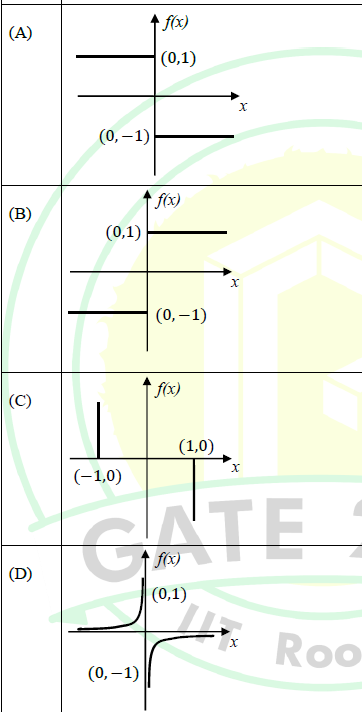
\includegraphics[width=0.3\columnwidth]{figs/Q.5.png}
        \caption{Four different plots of a function $f(x)$ versus $x$.}
        \label{fig:Q.5}
    \end{figure}
\end{enumerate}

\textbf{Q.6 - Q.10 Multiple Choice Question (MCQ), carry TWO marks each (for each wrong answer: $-2/3$).}
 
\begin{enumerate}
    \setcounter{enumi}{5}
    \item Identify the option that has the most appropriate sequence such that a coherent paragraph is formed:
    \\
    P. Over time, such adaptations lead to significant evolutionary changes with the potential to shape the development of new species.
\\
    Q. In natural world, organisms constantly adapt to their environments in response to challenges and opportunities.
\\
    R. This process of adaptation is driven by the principle of natural selection, where favorable traits increase an organism's chances of survival and reproduction.
\\
    S. As environments change, organisms that can adapt their behavior, structure and physiology to such changes are more likely to survive.
\begin{multicols}{2}
    \begin{enumerate}
        \item $P \rightarrow Q \rightarrow R \rightarrow S$
        \item $Q \rightarrow S \rightarrow R \rightarrow P$
        \item $R \rightarrow S \rightarrow Q \rightarrow P$
        \item $S \rightarrow P \rightarrow R \rightarrow Q$
    \end{enumerate}
    \end{multicols}

    \item A stick of length one meter is broken at two locations at distances of $b_{1}$ and $b_{2}$ from the origin ($0$), as shown 
in the figure. Note that $0 < b_{1} < b_{2} < 1$.
Which one of the following is NOT a necessary condition for forming a triangle using the three pieces?
\begin{figure}[!h]
        \centering
        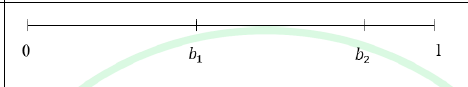
\includegraphics[width=0.3\columnwidth]{figs/Q.7.png}
        \caption{A one-meter stick broken at two points, $b_1$ and $b_2$, resulting in three pieces.}
        \label{fig:Q.7}
    \end{figure}
    \begin{multicols}{2}
    \begin{enumerate}
        \item $b_{1} < 0.5$
        \item $b_{2} > 0.5$
        \item $b_{2} < b_{1} + 0.5$
        \item $b_{1} + b_{2} < 1$
    \end{enumerate}
    \end{multicols}

    \item Eight students ($P$, $Q$, $R$, $S$, $T$, $U$, $V$, and $W$) 
are playing musical chairs. The figure indicates their order of position at the start of the game.
They play the game by moving forward in a circle in the clockwise direction.
After the $1^{st}$ round, $4^{th}$ student behind $P$ leaves the game.
After $2^{nd}$ round, $5^{th}$ student behind $Q$ leaves the game. After $3^{rd}$ round, $3^{rd}$ student behind $V$ leaves the game.
After $4^{th}$ round, $4^{th}$ student behind $U$ leaves the game.
Who all are left in the game after the $4^{th}$ round?
\begin{figure}[!h]
        \centering
        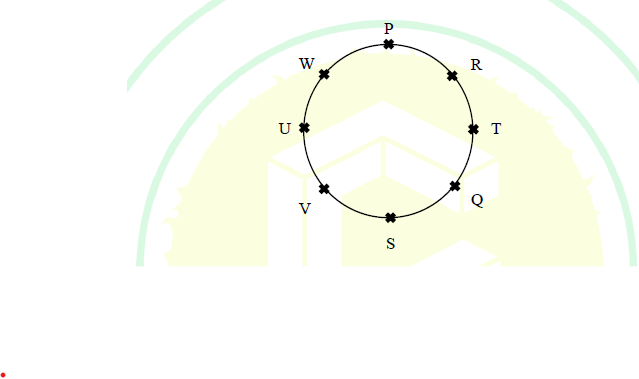
\includegraphics[width=0.2\columnwidth]{figs/Q.8.png}
        \caption{Initial clockwise arrangement of eight students (P, Q, R, S, T, U, V, W) for a game of musical chairs.}
        \label{fig:Q.8}
    \end{figure}
    \begin{multicols}{2}
    \begin{enumerate}
        \item $P$;
$T$; $Q$; $S$
        \item $V$; $P$; $T$;
$Q$
        \item $W$; $R$; $Q$;
        \item $Q$; $T$; $V$;
$W$
    \end{enumerate}
    \end{multicols}

    \item The table lists the top $5$ nations according to the number of gold medals won in a tournament;
also included are the number of silver and the bronze medals won by them.
Based only on the data provided in the table, which one of the following statements is INCORRECT?
\begin{center}
    \begin{tabular}{|l|c|c|c|}
        \hline
        \textbf{Nation} & \textbf{Gold} & \textbf{Silver} & \textbf{Bronze} \\ \hline
        USA & $40$ & $44$ & $41$ \\
        Canada & $39$ & $24$ & $27$ \\
        Japan & $12$ & $20$ & $13$ \\
        Australia & $19$ & $17$ & $16$ \\
        France & $16$ & 
$26$ & $22$ \\ \hline
    \end{tabular}
    \end{center}
    \begin{enumerate}
        \item France will occupy the third place if the list were made on the basis of the total number of medals won.
\item The order of the top two nations will not change even if the list is made on the basis of the total number of medals won.
\item USA and Canada together have less than $50$\% of the medals awarded to the nations in the above table.
\item Canada has won twice as many total medals as Japan.
\end{enumerate}

    \item An organization allows its employees to work independently on consultancy projects but charges an overhead on the consulting fee.
The overhead is $20$\% of the consulting fee, if the fee is up to $5,00,000$.
For higher fees, the overhead is $1,00,000$ plus $10$\% of the amount by which the fee exceeds $5,00,000$.
The government charges a Goods and Services Tax of $18$\% on the total amount (the consulting fee plus the overhead).
An employee of the organization charges this entire amount, i.e., the consulting fee, overhead, and tax, to the client.
If the client cannot pay more than $10,00,000$, what is the maximum consulting fee that the employee can charge?
\begin{multicols}{2}
    \begin{enumerate}
        \item $7,01,438$
        \item $7,24,961$
        \item $7,51,232$
        \item $7,75,784$
    \end{enumerate}
    \end{multicols}
\end{enumerate}
\clearpage

\section*{\textbf{Ecology and Evolution (EY)}}
\textbf{Q.11 - Q.35 Carry ONE mark Each}
\begin{enumerate}
\setcounter{enumi}{10}
    \item In a linear regression, a line of best fit can be obtained by
    \begin{enumerate}
        \item minimizing the sum of squares of the residuals
      
  \item minimizing the sum of the residuals
        \item minimizing the standard deviation from the mean
        \item minimizing the standard error of the mean
    \end{enumerate}

    \item Fly larvae of a species feed simultaneously on a shared rotting fruit.
If the density of fly larvae is high, then all the larvae grow up to be smaller sized adults than if the larval density were low.
Which one of the following processes best describes this observation?
\begin{multicols}{2}
    \begin{enumerate}
        \item Scramble competition
        \item Interspecific competition
        \item Competitive exclusion
        \item Apparent competition
    \end{enumerate}
    \end{multicols}
    
    \item In primates, males are often larger than females.
If sexual dimorphism evolved to enable males to compete for access to multiple females, in which mating system would we expect to see the greatest sexual dimorphism?
\begin{multicols}{2}
    \begin{enumerate}
        \item Monogamy
        \item Polygyny
        \item Polyandry
        \item Parthenogamy
    \end{enumerate}
    \end{multicols}

    \item Hosts of parasites evolve effective immune responses to infection, which in turn results in those parasites evolving increased infectiousness towards the hosts.
Which one of the following processes describes this type of interaction between hosts and parasites?
\begin{multicols}{2}
    \begin{enumerate}
        \item Co-evolution
        \item Quorum sensing
        \item Convergent evolution
        \item Character displacement
    \end{enumerate}
    \end{multicols}

    \item Male rhinoceros beetles have horns that they use to fight each other.
Despite the competitive advantage of having large horns, horn length never exceeds two thirds of their body length.
What form of selection explains why horn length is constrained?
\begin{multicols}{2}
    \begin{enumerate}
        \item Directional selection
        \item Disruptive selection
        \item Artificial selection
        \item Stabilizing selection
    \end{enumerate}
    \end{multicols}

    \item Lizards that produce many eggs often have a shorter lifespan than those who produce fewer eggs.
Which one of the terms below describes the relationship between the number of eggs and lifespan?
\begin{multicols}{2}
    \begin{enumerate}
        \item Compensatory growth
        \item Frequency dependent selection
        \item Biomagnification
        \item Life-history tradeoff
    \end{enumerate}
    \end{multicols}

    \item A butterfly species in a homogenous forest patch starts exhibiting assortative mating, such that spotted individuals always mate with each other and plain individuals always mate with each other.
This trait is heritable, and spotted parents always produce spotted offspring and plain parents always produce plain offspring.
Which one of the following forms of speciation could this prezygotic reproductive barrier most likely lead to?
\begin{multicols}{2}
    \begin{enumerate}
        \item Sympatric speciation
        \item Cryptic speciation
        \item Allopatric speciation
        \item Peripatric speciation
    \end{enumerate}
    \end{multicols}

    \item The hippocampus is a region of the brain whose size is positively correlated with navigation and spatial mapping ability in birds and mammals.
Which one of the following observations would NOT be consistent with this statement?
\begin{enumerate}
        \item When the size of the hippocampus is surgically reduced in laboratory rats, their ability to find food is reduced in a radial arm maze
        \item Bird species that hoard food in different parts of their territory have a larger hippocampus than similarly-sized bird species that do not hoard food
        \item In domestic pigeons, non-homing varieties have a larger hippocampus than homing varieties
        \item In voles, males have larger home ranges 
than females, and the hippocampus of males is larger than that of females
    \end{enumerate}

    \item A bird eats two types of worms, $P$ and $Q$, picking them randomly.
Which one of the following describes the kind of probability distribution of the number of worms of type $P$ eaten by the bird in a day?
\begin{multicols}{2}
    \begin{enumerate}
        \item Binomial
        \item Normal
        \item Log-normal
        \item Uniform
    \end{enumerate}
    \end{multicols}

    \item Which one of the following is an example of a cell type found only in a single phylum?
\begin{multicols}{2}
    \begin{enumerate}
        \item Cnidocyte
        \item Erythrocyte
        \item Myocyte
        \item Neurocyte
    \end{enumerate}
    \end{multicols}
    
    \item Fossils of most of the modern animal phyla first appeared over a short period of time.
In which one of the following geological time periods did this occur?
\begin{multicols}{2}
    \begin{enumerate}
        \item Cambrian
        \item Cretaceous
        \item Jurassic
        \item Permian
    \end{enumerate}
    \end{multicols}
    
    \item Certain species of ibex and weevils depend on the same food source.
A study finds that the removal of ibex results in an increase in the number of weevils, but the removal of weevils does not affect the ibex.
Which one of the following options best describes this interaction?
\begin{multicols}{2}
    \begin{enumerate}
        \item Amensalism
        \item Commensalism
        \item Mutualism
        \item Parasitism
    \end{enumerate}
    \end{multicols}
    
    \item Across trophic levels, energy flows from producers to primary consumers, and from primary consumers to secondary consumers.
Which one of the following options best represents the percentage of energy that is transferred from producers to secondary consumers?
\begin{enumerate}
        \item Between $0.01$ and $0.02$ \%
        \item Between $0.5$ and $1.5$ \%
        \item Between $7.5$ and $12.5$ \%
        \item Between $72.5$ and $77.5$ \%
    \end{enumerate}
    
    \item High water temperatures can cause coral bleaching, which often leads to coral death.
In coral reefs that experience repeated bleaching, there can be substantial algal growth on dead coral, eventually leading to an algal dominated ecosystem.
Such a transformation is known as
    \begin{multicols}{2}
    \begin{enumerate}
        \item adaptive radiation
        \item coral transplantation
        \item coral recruitment
        \item phase shift
    \end{enumerate}
    \end{multicols}
    
    \item The species richness of trees increases from North to South in the Western Ghats, and from South to North in the Andes.
Which one of the following can be an explanation for these patterns?
\begin{enumerate}
        \item Greater incident solar radiation at lower latitudes
        \item Higher temperature at higher latitudes
        \item Greater distance from the coast at lower latitudes
        \item Stronger trade winds at higher latitudes
    \end{enumerate}
    
    \item Local communities are comprised of a subset of species from the regional species pool.
Which one of the following processes is LEAST likely to cause species composition of local communities to differ from one another?
\begin{enumerate}
        \item Local interspecific competition
        \item Regionally stable climatic conditions
        \item Stochastic demographic variation
        \item Local predator-prey interactions
    \end{enumerate}
    
    \item In this figure, the rectangle ($P$) depicts the range of temperature and rainfall in which a plant species can survive and propagate.
The circle ($Q$) demarcates the range of temperature and rainfall in which this plant species is actually found.
Which one of the following statements about $P$ and $Q$ is accurate for this plant species?
\clearpage
\begin{figure}[!h]
        \centering
        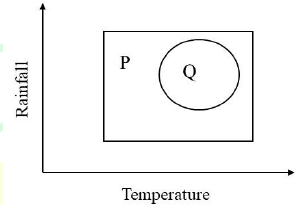
\includegraphics[width=0.5\columnwidth]{figs/Q.27.png}
        \caption{A plot showing the potential range (Rectangle P) and actual range (Circle Q) of a plant species based on temperature and rainfall.}
        \label{fig:Q.27}
    \end{figure}
    \begin{enumerate}
        \item $P$ is the fundamental niche and $Q$ is the realized niche
        \item $P$ is the fundamental niche and $Q$ is the habitat
        \item $Q$ is the fundamental niche and $P$ is the realized niche
        \item $Q$ is the fundamental niche and $P$ is the habitat
  
  \end{enumerate}
    
    \item Match the following geographic regions to the mammals that are native to those regions.
\begin{center}
    \begin{tabular}{ll}
        \textbf{Geographic regions} & \textbf{Mammals} \\
        (P) Western Ghats & (i) Golden langur \\
        (Q) Western Himalaya & (ii) Malabar giant squirrel \\
        (R) Northeast India & (iii) Pika \\
        (S) Andaman and Nicobar Islands & (iv) Nilgai \\
        & (v) Long-tailed macaque
    \end{tabular}
    \end{center}
    
\begin{multicols}{2}
    \begin{enumerate}
        \item P-iii; Q-ii; R-i;
S-v
        \item P-ii; Q-iii; R-i;
S-iv
        \item P-ii; Q-iii; R-i;
S-v
        \item P-iii; Q-v; R-ii;
S-iv
    \end{enumerate}
    \end{multicols}

    \item Mayflies lay eggs in water.
Their nymphs (immature life stage) are aquatic and adults are terrestrial.
Some mayflies perceive dry, paved parking lots as waterbodies and lay eggs there that do not survive.
In this situation, which one or more of these statements is/are correct?
\begin{enumerate}
        \item These parking lots are ecological sink habitats, whereas adjacent waterbodies are source habitats
        \item This is an example of antagonistic coevolution between humans and insects
        \item Mayflies have an iteroparous life history strategy
        \item Laying eggs in these parking lots instead of waterbodies would reduce the fitness of individual female mayflies
    \end{enumerate}

    \item Fish schools in coral reefs can comprise multiple species that swim 
and forage together. Which one or more of the following options describe(s) potential fitness benefit(s) to individuals in a mixed-species group?
\begin{enumerate}
        \item Individuals of some species draw the attention of predators away from the school, thereby sacrificing themselves for the survival of the group
        \item Some species join mixed-species groups in order to hybridize
        \item Larger groups reduce the per capita risk of predation
        \item Individuals of some species feed on the substrate, while others feed on the invertebrates that are flushed out by the substrate-feeder
    \end{enumerate}

   
 \item During migration, which one or more of the following do birds use for long-distance navigation?
\begin{multicols}{2}
    \begin{enumerate}
        \item Celestial cues
        \item Earth's magnetic field
        \item Chemical cues
        \item Polarized light
    \end{enumerate}
    \end{multicols}

    \item Which one or more of the following functions do insects directly perform in ecosystems?
\begin{multicols}{2}
    \begin{enumerate}
        \item Decomposition
        \item Pollination
        \item Photosynthesis
        \item Vernalization
    \end{enumerate}
    \end{multicols}

    \item In a lake with a large population of fish, there are $4$ blue fish for every red fish.
Every fish has an equal probability of being caught. If you dip a net into this lake and pick up $4$ individuals at random, the probability that you will get $2$ fish of each colour is \underline{\hspace{3cm}}.
(Round off to three decimal places)

    \item There are $9$ different rock lizard species, each with a unique colour.
Lizards of $2$ different species sit on a rock at any given time.
The number of possible colour combinations of rock lizards seen together on a rock is \underline{\hspace{3cm}}.
(Answer in integer)

    \item In a population of $534$ blue sheep, there are two alleles, $P$ and $Q$, at an autosomal locus.
Allele $P$ has a frequency of $30$\%. The number of sheep with the $QQ$ genotype is $262$.
Assuming that this population is at Hardy-Weinberg equilibrium, the expected percentage of sheep with the $PQ$ genotype in the population is \underline{\hspace{3cm}} \%.
(Round off to two decimal places)
\end{enumerate}

\textbf{Q.36 - Q.65 Carry TWO marks Each}
\begin{enumerate}
    \setcounter{enumi}{35}
    \item Rotting leaves of mango are composed of $25$\% of compound $P$ which decomposes exponentially at a rate $k_P = 0.5 \text{ yr}^{-1}$ and $75$\% of compound $Q$ which decomposes exponentially at a rate $k_Q = 0.1 \text{ yr}^{-1}$.
What percentage of the initial amount of compound $Q$ remains when half of the initial amount of compound $P$ has decomposed?
Choose the closest numerical value from the options provided.
    \begin{multicols}{2}
    \begin{enumerate}
        \item $87$\%
        \item $50$\%
        \item $75$\%
        \item $37$\%
    \end{enumerate}
    \end{multicols}

    \item The origin and proliferation of which one of the following organisms was responsible for the 'Great Oxidation Event'?
\begin{multicols}{2}
    \begin{enumerate}
        \item Cyanobacteria
        \item Fungi
        \item Plants
        \item Virus
    \end{enumerate}
    \end{multicols}

    \item Which one of the following mechanisms is expected to generate tightly linked genes?
\begin{multicols}{2}
    \begin{enumerate}
        \item Chromosomal inversion
        \item Deletion of an exon
        \item Gene duplication
        \item Insertion of an exon
    \end{enumerate}
    \end{multicols}

    \item Newts produce tetrodotoxin ($TTX$), a poison that targets sodium ion channels, for defense against their predators, garter snakes.
Several species of garter snakes are resistant to newt $TTX$ due to specific known amino acid substitutions in garter snake sodium channels.
Which one of the following is best-suited to identify whether this adaptation in garter snakes has a single origin or multiple independent origins?
\begin{enumerate}
        \item Building a gene phylogeny of sodium ion channel in garter snakes
        \item Building a species phylogeny of garter snakes
        \item Building a gene phylogeny of newt sodium ion channels and species phylogeny of newts, and comparing them
        \item Building a gene phylogeny of garter snake sodium ion channels and a species phylogeny of garter snakes, and comparing them
    \end{enumerate}

    \item Many insect species carry 
the endosymbiotic bacteria Wolbachia, which are maternally inherited. Wolbachia persist over time in these insect hosts by increasing the fitness of the infected host.
This increased host fitness can lead to the fixation of Wolbachia in the host population, wherein all individuals carry it.
Which one of the following statements describes a process that would NOT allow Wolbachia to become fixed in the host population?
\begin{enumerate}
        \item Wolbachia induce cytoplasmic incompatibility and so, mating between infected and uninfected host individuals produces no viable offspring
        \item Wolbachia increase the fecundity of the host by increasing its longevity
        \item Wolbachia increase the immune response of the host to other infections
        \item Wolbachia induce cytoplasmic compatibility and so, only mating between infected and uninfected host individuals produces viable offspring
    \end{enumerate}
    
    
\item Figure $F$ shows how predation rate changes with increasing prey density.
Which one of the figures represents the per capita death rate of prey under the conditions of $F$?
\begin{figure}[!h]
        \centering
        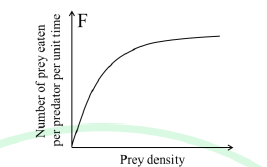
\includegraphics[width=0.3\columnwidth]{figs/Q.41-a.png}
        \caption{Plots showing predation dynamics. Plot F shows predation rate vs. prey density. Plots G, H, I, and J show different potential relationships for per capita death rate of prey vs. prey density.}
        \label{fig:Q.41-a}
    \end{figure}
\begin{figure}[!h]
        \centering
        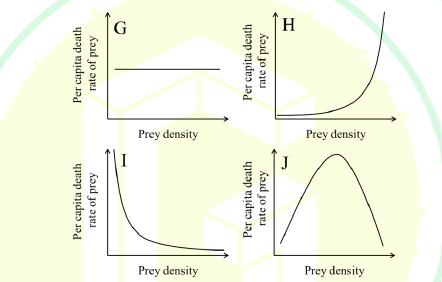
\includegraphics[width=0.3\columnwidth]{figs/Q.41-b.png}
        \caption{}
        \label{fig:Q.41-b}
    \end{figure}
    
    \begin{multicols}{4}
    \begin{enumerate}
        \item $G$
        \item $H$
        \item $I$
        \item $J$
    \end{enumerate}
    \end{multicols}
    
    \item Fungus $S$ infects elm trees and fungus $T$ infects chestnut trees, and both kill their hosts within a year 
of infection. A forest with equal density of elm and chestnut trees is colonized by both pathogenic fungi.
A $100$ years later, the elm tree population has declined and the chestnut trees have become extinct.
Which one of the following mechanisms would NOT contribute to this outcome?
\begin{enumerate}
        \item Fungus $S$ is dispersed by flightless beetles and fungus $T$ disperses by wind
        \item Elm trees reproduce much more quickly than chestnut trees
        \item Elm seeds disperse far away from the parent, while chestnut seeds fall near the parent
        \item Fungus $S$ reproduces much more quickly than fungus $T$
    \end{enumerate}
    
    \item The table below provides a list of study questions 
($P$, $Q$, $R$) and statistical tests (i, ii, iii).
    \begin{center}
    \begin{tabular}{|l|l|}
        \hline
        \textbf{Study question} & \textbf{Statistical Test} \\ \hline
        (P) Does flower colour follow & (i) Student's t-test \\ 
        Mendelian inheritance?
& \\ \hline
        (Q) Does increased visitation by & (ii) Chi-square test \\ 
        pollinators increase the number of viable & \\
        fruits produced by an individual?
& \\ \hline
        (R) Does the quantity of nectar & (iii) Pearson's correlation \\ 
        production differ between flowers that & analysis \\
        were visited by pollinators compared to & \\
        those that had no pollinator visitation?
& \\ \hline
    \end{tabular}
    \end{center}
    Which one of the following options correctly matches the study question to the most appropriate statistical test?
\begin{multicols}{2}
    \begin{enumerate}
        \item P-i; Q-ii;
R-iii
        \item P-i; Q-iii;
R-ii
        \item P-ii; Q-i;
R-iii
        \item P-ii; Q-iii;
R-i
    \end{enumerate}
    \end{multicols}
    
    \item A researcher wants to estimate the number of crickets in an isolated valley.
They captured $56$ crickets in the first session, and then marked and released them.
In the second session, they captured $41$ crickets of which $8$ were already marked.
Assuming that there is no birth, death, immigration or emigration in the cricket population during the study period, what is the estimated number of crickets in this valley?
\begin{multicols}{2}
    \begin{enumerate}
        \item $97$
        \item $247$
        \item $287$
        \item $334$
    \end{enumerate}
    \end{multicols}
    
    \item The table below lists potential environmental conditions in future climates, related to atmospheric carbon dioxide concentrations ($CO_2$) and mean annual temperature ($MAT$).
The table also lists potential outcomes with respect to whether conditions will favour grasses with C3 or C4 photosynthetic pathways.
Assuming no other changes in environmental conditions, match the options in the two columns.
\begin{center}
    \begin{tabular}{|l|l|}
        \hline
        \textbf{Environmental conditions} & \textbf{Outcomes} \\ \hline
        (P) Increased $CO_2$, no change in $MAT$ & (i) C3 performs better than C4 \\
        (Q) No change in $CO_2$, increased $MAT$ & (ii) C4 performs better than C3 \\
         & (iii) C3 and C4 perform equally \\ \hline
    \end{tabular}
    \end{center}
    \begin{multicols}{2}
  
  \begin{enumerate}
        \item P-i;
Q-iii
        \item P-i; Q-ii
        \item P-ii;
Q-iii
        \item P-iii;
Q-ii
    \end{enumerate}
    \end{multicols}
    
    \item In a grassland ($P$), there are $8$ plant species with a similar number of individuals of each species.
In another grassland ($Q$), there are $12$ species with uneven abundances.
Which one of the following statements about the Shannon's diversity index of $P$ and $Q$ is correct?
\begin{enumerate}
        \item The diversity index of $P$ is greater than $Q$
        \item The diversity index of $P$ is less than $Q$
        \item The diversity index of $P$ is equal to $Q$
        \item There is not enough information to draw a conclusion
    \end{enumerate}
    
    \item Which one of the following statements about genetic drift is accurate?
\begin{enumerate}
        \item Like mutation, drift increases genetic variation within a population
        \item Drift typically increases genetic differences between populations
        \item Drift typically reinforces the effects of natural selection in populations
        \item Drift increases with population size, leading to faster evolution
    \end{enumerate}
    
    \item Mean global temperature since pre-industrial times has increased approximately by
    \begin{multicols}{2}
    \begin{enumerate}
   
     \item $0$ to $0.5$ \textcelsius
        \item $1$ to $1.5$ \textcelsius
        \item $2$ to $3$ \textcelsius
        \item $3$ to $5$ \textcelsius
    \end{enumerate}
    \end{multicols}
    
    \item In a deer species that lives in groups, some individuals act as sentinels and are vigilant for predators but there is a trade-off between foraging and vigilance.
A researcher collects data on the foraging rates of edge (black) and central (grey) members of the group in two similar forests, one with and one without predators.
Which one of the following figures best supports the hypothesis that members at the edge are acting as sentinels in this deer species?
\clearpage
\begin{figure}[!h]
        \centering
        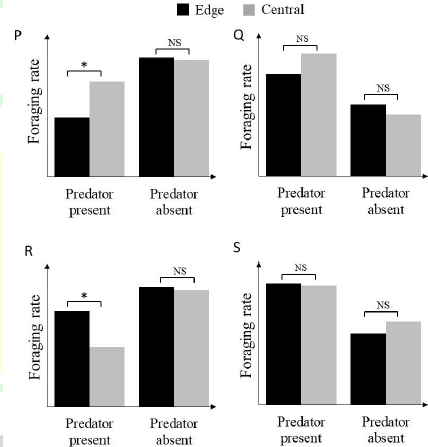
\includegraphics[width=0.6\columnwidth]{figs/Q.49.png}
        \caption{Four possible outcomes (P, Q, R, S) for foraging rates of deer at the edge (black bars) and center (grey bars) of a group, in habitats with and without predators.}
        \label{fig:Q.49}
    \end{figure}
    \begin{multicols}{4}
    \begin{enumerate}
        \item $P$
        \item $Q$
        \item $R$
        \item $S$
    \end{enumerate}
    \end{multicols}
    
    \item A patch of forest (I) has been declared as a protected area.
Conservationists have surveyed three other patches of forest (II, III and IV) and can only recommend one of them for protection.
In the figure below, each letter denotes a different species of frog.
The conservationists recommend that Patch IV should be protected. Which one of the following metrics is this decision based on?
\begin{figure}[!h]
        \centering
        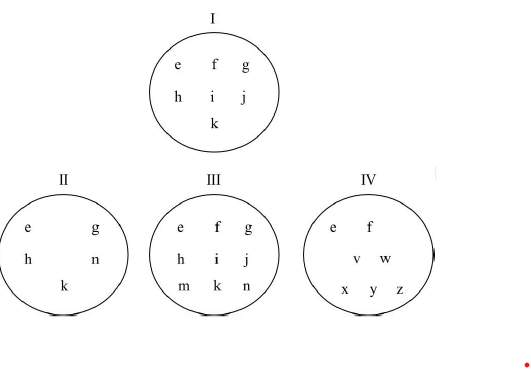
\includegraphics[width=0.4\columnwidth]{figs/Q.50.png}
        \caption{Species composition of frogs (denoted by letters) in four different forest patches (I, II, III, IV).}
        \label{fig:Q.50}
    \end{figure}
    \begin{multicols}{2}
    \begin{enumerate}
        \item Species richness
        \item Complementarity
        \item Alpha diversity
        \item Evenness
    \end{enumerate}
    \end{multicols}
    
    \item The numbers of rabbits ($R$) and their predators, foxes ($F$), in an ecosystem are modelled by the 
Lotka-Volterra equations as follows:
    $$ \frac{dR}{dt} = 2R - 0.01 RF $$
    $$ \frac{dF}{dt} = -F + 0.005 RF $$
    where the time is measured in months.
If there are currently $100$ rabbits and $10$ foxes, the number of rabbits is changing at the rate of \underline{\hspace{2cm}} per month and the number of foxes is changing at the rate of \underline{\hspace{2cm}} foxes per month.
\begin{multicols}{2}
    \begin{enumerate}
        \item $+190$ and $-5$
        \item $+5$ and $-190$
        \item $-190$ and $+5$
        \item $-10$ and $+5$
    \end{enumerate}
    \end{multicols}

    \item The number of species found on islands typically increases with the size of the island.
Which one or more of the following options explains this relationship between island size and species richness?
\begin{enumerate}
        \item Large islands have more habitat types than small islands
        \item Large islands are colonized by more species than small islands
        \item Small islands have higher species extinction rates than large islands
        \item Small islands are closer to the mainland than large islands
    \end{enumerate}
    
    \item Decreasing surface area to volume ratio helps reduce heat loss in colder climates.
In which one or more of the following observations does this play a role?
\begin{enumerate}
        \item Related species of mammals are larger in size at higher latitudes
        \item Birds lay more clutches of eggs at higher latitudes
        \item Birds and mammals huddle tightly together at higher latitudes
        \item Mammals have longer limbs and larger ears at higher latitudes
    \end{enumerate}
    
    \item The table below describes the number of tree species in a forest whose seeds are dispersed 
by large or small animals, and whether they are insect or wind pollinated.
In the past, seed dispersers and pollinators were abundant in this forest.
Now, there are very few large animal dispersers, but the number of small animal dispersers has not changed.
There are also very few insect pollinators in this forest.
Which one or more of the following inferences about trees in the forest can be drawn from these changes in seed dispersers and pollinators?
\begin{center}
    \begin{tabular}{|l|c|c|}
    \hline
    & \textbf{Insect pollinated} & \textbf{Wind pollinated} \\ \hline
    \textbf{Dispersed by large animals} & $85$ tree species & $19$ tree species \\ \hline
    \textbf{Dispersed by small animals} & $25$ tree species & $11$ tree species \\ \hline
    \end{tabular}
    \end{center}
    \begin{enumerate}
        \item Mortality of all trees in this forest will decrease in the future
        \item Mortality of a large number of 
trees in this forest will increase in the future
        \item Regeneration of all tree species in this forest will increase in the future
        \item Regeneration of a large number of tree species will decrease in future
    \end{enumerate}

    \item Which one or more of the following would make a plant community more susceptible to invasion by exotic plants?
\begin{enumerate}
        \item Anthropogenic influx of nutrients
        \item Decline in density of a dominant species due to disease
        \item Arrival of a highly competitive exotic species
        \item Absence of suitable pollinators for an invading species
    \end{enumerate}
    
    \item Aphids feed on both alfalfa and clover plants.
A researcher collected and reared different genotypes of aphids from separate alfalfa and clover fields.
He then measured the fecundity of both aphid groups when fed on each of the two host plants.
The figure summarizes the performance of aphid groups originating from alfalfa (dashed) or clover (solid).
Which one or more of the following situations does the figure depict?
\begin{figure}[!h]
        \centering
        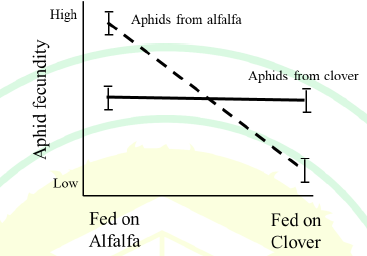
\includegraphics[width=0.4\columnwidth]{figs/Q.56.png}
        \caption{Fecundity of aphids originating from alfalfa (dashed line) and clover (solid line) when reared on both alfalfa and clover host plants.}
        \label{fig:Q.56}
    \end{figure}
    \begin{enumerate}
        \item Aphids demonstrate a genotype by environment interaction
        \item Aphids from clover fields are much less genetically variable than aphids from alfalfa fields
        \item Aphids from clover fields are locally adapted to their original host
        \item Aphids from clover fields show high plasticity
    \end{enumerate}
 
   
    \item Which one or more of the following processes has/have resulted in increased greenhouse gases in the atmosphere over the last $100$ years?
\begin{enumerate}
        \item Increasing levels of $N_2$ in the atmosphere due to increased denitrification
        \item Increased release of $CO_2$ into the atmosphere due to the burning of fossil fuels
        \item Increased release of methane into the atmosphere due to livestock
        \item Increased release of methane from wetlands soil
    \end{enumerate}
    
    \item The figure below shows the reproductive success of two alternative mating strategies, with 
respect to their frequency in the population. Territorial males (solid line) defend territories to get mates, and Sneaker males (dashed line) obtain mating opportunities without having territories.
Which one or more of the following conclusions can be drawn from this figure?
\begin{figure}[!h]
        \centering
        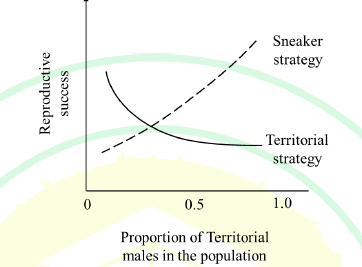
\includegraphics[width=0.4\columnwidth]{figs/Q.58.png}
        \caption{Reproductive success as a function of frequency in the population for two alternative mating strategies: Territorial males (solid line) and Sneaker males (dashed line).}
        \label{fig:Q.58}
    \end{figure}
    \begin{enumerate}
        \item The reproductive success of Territorial and Sneaker males can never be the same in the population
        \item The reproductive success of Sneaker males is influenced by the proportion of Territorial males in the population
        \item The highest possible reproductive success can be obtained by Sneaker males, and not Territorial males
    
    \item Territorial males will always have a higher reproductive success than Sneaker males
    \end{enumerate}
    
    \item From the table below, choose one or more of the options that match(es) the evolutionary biologists with the organisms they are well-known to have studied.
\begin{center}
    \begin{tabular}{|l|l|} \hline
    \textbf{Evolutionary biologist} & \textbf{Organism} \\ \hline
    (P) Charles Darwin & (i) Mountain gorilla \\
    (Q) Gregor Mendel & (ii) Giant tortoise \\
    (R) Dian Fossey & (iii) Finches \\
    (S) Frederick Griffith & (iv) Pea plant \\ 
    & (v) Streptococcus pneumoniae \\ \hline
    \end{tabular}
    \end{center}
    \begin{multicols}{2}
    \begin{enumerate}
        \item P-ii;
Q-iv; R-i; S-v
        \item P-ii; Q-iv; R-ii;
S-iv
        \item P-iii; Q-iv; R-i;
S-v
        \item P-v; Q-i; R-v;
S-iii
    \end{enumerate}
    \end{multicols}
    
    \item Consider the following figure of sequence divergence over time.
The dashed and solid lines represent synonymous and non-synonymous substitutions, respectively.
Which one or more of the following does the figure support?
\begin{figure}[!h]
        \centering
        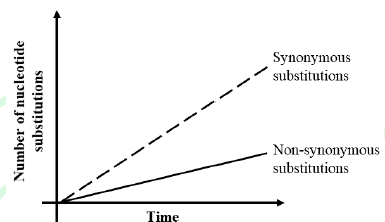
\includegraphics[width=0.4\columnwidth]{figs/Q.60.png}
        \caption{Sequence divergence over time, showing the rate of synonymous substitutions (dashed line) and non-synonymous substitutions (solid line).}
        \label{fig:Q.60}
    \end{figure}
    \begin{enumerate}
        \item Adaptive evolution
        \item Molecular clock
        \item Neutral theory of evolution
        \item Positive selection
    \end{enumerate}
    
    \item Modern humans of European descent have a much higher proportion of Neanderthal DNA than modern humans of African descent.
Which one or more of the following statements is/are consistent with this information?
\begin{enumerate}
        \item Following the migration of Neanderthals out of Africa into Europe, modern humans, who were already present in Europe, bred with them
        \item Following the migration of modern humans out of Africa into Europe, Neanderthals, who were already present in Europe, bred with them
        \item Modern humans and Neanderthals bred in Africa and then migrated out of Africa into Europe
        \item Modern humans and Neanderthals did not interbreed
    
\end{enumerate}
    
    \item A phylogenetic tree representing the evolutionary relationship between various vertebrates is shown below.
Given this tree topology, which one or more of the following statements is/are correct?
\begin{figure}[!h]
        \centering
        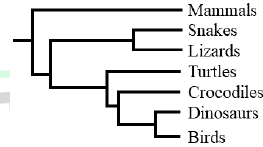
\includegraphics[width=0.4\columnwidth]{figs/Q.62.png}
        \caption{A phylogenetic tree illustrating the evolutionary relationships among various vertebrate groups, including mammals, turtles, crocodiles, dinosaurs, and birds.}
        \label{fig:Q.62}
    \end{figure}
    \begin{enumerate}
        \item Crocodiles are more closely related to turtles than they are to dinosaurs
        \item Mammals represent the outgroup with respect to reptiles
        \item Dinosaurs are more closely related to crocodiles than they are to birds
        \item Reptiles are nested within mammals
    \end{enumerate}
   
 
    \item The population of whirligig beetles in a lake grows or declines exponentially i.e. $ N(t) = N(0)e^{rt} $ where $N(t)$ is the population size at time $t$, $N(0)$ is the initial population size and $r$ is the per capita rate of population change, occurring only due to birth and death.
A researcher tracks population sizes for a year and finds the following:
    \begin{center}
    \begin{tabular}{|l|c|c|}
    \hline
    %hy\-phen\-ation
    \textbf{Time interval} & \textbf{Number of beetles at start} & \textbf{Number of beetles at end} \\ \hline
    January - March & $1000$ & $150$ \\
    April - June & $150$ & $3013$ \\
    July - September & $3013$ & $100$ \\
    October - December & $100$ & $2009$ \\ \hline
    \end{tabular}
    \end{center}
    Assuming 
that the individual birth rates remain constant throughout the year and only death rates are affected, which one or more of the following statements is/are true?
(In your calculations, round off the birth and date rates to two decimal places)
    \begin{enumerate}
        \item The death rate during April-June is equal to that during October-December
        \item The death rate during July-September is lower than that during January-March
        \item The death rate during July-September is higher than that during January-March
        \item The death rate during April-June is higher than that during October-December
    \end{enumerate}
   
 
    \item Which one or more of the following conditions is/are necessary for the evolution of increased nectar production in an insect-pollinated plant via natural selection?
\begin{enumerate}
        \item Increased nectar production in individual plants results in greater fruit set and number of offspring for these individuals
        \item The quantity of nectar produced by flowers varies across individuals in the population
        \item The quantity of nectar produced by a flower increases when more pollinators visit that same flower
        \item The quantity of nectar produced is heritable, i.e. passed on from parent to offspring
    \end{enumerate}

   
 \item The following empirical relationship describes how the number of trees $N(t)$ in a patch changes over time ($t$)
    $$ N(t) = -2t^2 + 12t + 24 $$
    where $t = 0$ is when the number of trees were first counted.
Given this relationship, the maximum number of trees that occur in the patch is \underline{\hspace{3cm}}.
(Round off to the nearest integer)
\end{enumerate}
\bigskip
\centering {\textbf{\large{END OF QUESTION PAPER}}}

\end{document}